\documentclass{article}


\usepackage[round]{natbib}
\usepackage{amsmath,amssymb,amsthm,bm,enumerate,mathrsfs,mathtools}
\usepackage{latexsym,color,verbatim,multirow}
\usepackage{graphicx}
\usepackage{caption}
\usepackage{subcaption}
\usepackage{tikz}
\usepackage{geometry}
\usetikzlibrary{shapes,arrows}
\tikzstyle{block} = [rectangle, draw, fill=white!20,
    text width=7em, text centered, rounded corners, minimum height=4em]
\tikzstyle{title} = [text width=7em, text centered, font=\bfseries]
\tikzstyle{line} = [draw, -latex']


\usepackage{mycommands}

\begin{document}

\newtheorem{theorem}{Theorem}
\newtheorem{corollary}[theorem]{Corollary}
\newtheorem{lemma}[theorem]{Lemma}
\newtheorem{observation}[theorem]{Observation}
\newtheorem{proposition}[theorem]{Proposition}
\newtheorem{definition}[theorem]{Definition}
\newtheorem{claim}[theorem]{Claim}
\newtheorem{fact}[theorem]{Fact}
\newtheorem{assumption}[theorem]{Assumption}
\newtheorem{model}[theorem]{Model}

\theoremstyle{definition}
\newtheorem{example}{Example}

\newcommand{\cM}{\mathcal{M}}
\newcommand{\cH}{\mathcal{H}}
\newcommand{\cD}{\mathcal{D}}
\newcommand{\FDR}{\textnormal{FDR}}
\newcommand{\FCR}{\textnormal{FCR}}
\newcommand{\crt}{\phi}
\newcommand{\M}{\mathcal{M}}
\newcommand{\cY}{\mathcal{Y}}
\newcommand{\cX}{\mathcal{X}}
\newcommand{\cV}{\mathcal{V}}
\newcommand{\bX}{\mathbf{X}}
\newcommand{\x}{\mathbf{x}}
\newcommand{\Gv}{\;\;\big|\;\;}
%\newcommand{\cP}{\mathcal{P}}
\newcommand{\proj}{\cP}
\newcommand{\pow}{\text{Pow}}
\newcommand{\sF}{\mathscr{F}}
\newcommand{\cF}{\mathcal{F}}
\newcommand{\sC}{\mathscr{C}}
\newcommand{\hJ}{\widehat{J}}
\newcommand{\bH}{\mathbf{H}}
\newcommand{\bM}{\mathbf{M}}
\newcommand{\tM}{\widetilde{M}}
\newcommand{\tE}{\widetilde{E}}
\newcommand{\tV}{\widetilde{V}}
\newcommand{\tR}{\widetilde{R}}
\newcommand{\tL}{\widetilde{L}}
\newcommand{\hk}{\hat{k}}
\newcommand{\hr}{\hat{r}}
\newcommand{\cN}{\mathcal{N}}
\newcommand{\leqAS}{\overset{\textrm{a.s.}}{\leq}}


\newcommand*\mystrut{\vrule width0pt height0pt depth1.5ex\relax}
\newcommand{\underlabel}{\underbracket[1pt][.5pt]{\mystrut \quad\;\; \sub \quad\;\; }}
\newcommand{\JTcomment}[1]{{\color{blue}{(JT: \bf \sc #1) }}}
\newcommand{\WFcomment}[1]{{\color{red}{(WF: \bf \sc #1) }}}

\title{Adaptive Sequential Model Selection}
\author{William Fithian, Jonathan Taylor, Rob Tibshirani, and Ryan Tibshirani}
\maketitle

\begin{abstract}
  Many model selection algorithms produce a ``path'' of fits that can be veiwed as specifying a sequence of models of increasing complexity. Given such a sequence of models and the data set used to produce them, we consider the problem of choosing the least complex model that is not falsified by the data, while accounting for the fact that the model path is determined adaptively using the data. Extending the tools of Fithian, Sun and Taylor (2014), we construct a $p$-value for each step in the sequence. In the case of linear regression, our $p$-values improve on the power of the spacings test of \citet{taylor2014exact}, often dramatically. By combining our $p$-values with stopping rules proposed by \citet{gsell2013sequential}, we achieve adaptive control of the familywise error rate and false discovery rate.
\end{abstract}


\section{Introduction}

... generates a sequence of increasingly complex models. Our goal is to choose the simplest model that is not falsified by the available data.

... and find the index of the smallest adequate model --- that is, the smallest model that cannot be falsified given available evidence.

\begin{example}[Forward-Stepwise Linear Regression with the LASSO]
  \citet{taylor2014exact}
\end{example}

\begin{example}[The LARS Algorithm in Regression]
  \citet{taylor2014exact}
\end{example}

\begin{example}[Ever-Active Path in $\ell_1$-Regularized Methods]
  \citet{taylor2014exact}
\end{example}

\begin{example}[Principal Components Analysis]
  As a second motivating example, consider model selection for   principal components analysis. In that case we are given a data matrix $X \in \R^{n\times d}$, with which we form a sample covariance matrix
\[
S = \frac{1}{n-1} \sum_{i=1}^n(x_i - \bar x)^2
\]
The first $d$ principal component loadings are the first $d$ eigenvectors of $S$, which call $u_1,\ldots, u_d$. These induce a sequence of nested Wishart models:
\[
M_0 \sub M_1 \sub \cdots \sub M_d
\]
in which
\begin{equation}
  M_k:\; (n-1) S \sim W_d\left(\lambda_0 I_d + \sum_{\ell=1}^k     \lambda_\ell u_i u_i', \;\;\; n-1\right).
\end{equation}
This problem was studied in \citet{choi2014selecting}.
\end{example}

\subsection{Generic Setting}

More generically, we observe data $Y \in \cY$, with unknown sampling distribution $F$. We then use $Y$ to generate an adaptive sequence of $d$ nested models
\[
M_0(Y) \sub M_1(Y) \sub \cdots \sub M_d(Y).
\]
Define the {\em completion index} $k_0(Y) = \min\{k:\; F \in M_k\}$, the index of the first correct model. 

We will consider two related problems. First, we will consider the problem of obtaining selective single-step $p$-values, where $p_k$ is a $p$-value for testing
\[
H_{0,k}:\; F\in M_{k-1}\quad \text{ vs. } \quad 
H_{1,k}:\; F\in M_k\setminus M_{k-1},
\]
while adjusting for the fact that the models are chosen adaptively. As we will see, {\em selected-model} tests can be dramatically more powerful than {\em saturated-model} tests at early steps in the model path when most of the signal variables have not yet entered the model.

The second half of the paper concerns {\em stopping rules} $\hk$, estimators of $k_0$. We will consider several stopping rules that operate on the full sequence $p_{[d]}$, including two powerful stopping rules proposed in \citet{gsell2013sequential}. These latter require guarantees on the joint law of the $p$-values. We will prove sufficient conditions for when the $p$-values are Gaussian.

Although we will focus most of our attention and examples on the case of selecting a set of predictors in linear regression, essentially all of our results apply in generic exponential family models.

\subsection{Which Null Hypothesis Should We Test?}

There is some ambiguity involved in deciding how to generalize $z$- and $t$-tests to the selective case. For example, \citet{gsell2013sequential} describe three different null hypotheses that we could consider testing at step $k$. As discussed at some length in \citet{fithian2014optimal}, there are several different models that 

In some cases the design matrix of the full model may represent a  scrupulously curated set of features, and the analysts may know in advance that inferences with respect to the full model are of major scientific interest. For example, the scientist may believe, due to theoretical considerations, that a nonzero coefficient of $X_1$ after controlling for $X_2,\ldots,X_p$ would be evidence for a causal effect of $X_1$ on the response.

If the full model has no special scientific status, however, then we see little advantage in insisting that all inferences should adjust for every other predictor in the full design matrix $X$. For example, suppose that $X$ contains gene expression measurements for all genes that happened to be measured by a microarry chip. Then $\beta_{j,\text{Full}}$ is already fairly arbitrary, since we would be controlling for a different set of genes if we had purchased the chip from a different manufacturer.

\WFcomment{Also say: Controlling for more variables could take us farther from a causal effect; furthermore, coefficient in larger model is much harder to interpret.}


\section{Inference for One Step}

To begin, we consider the problem of constructing a valid selective $p$-value for a particular step. At step $k$, we construct $p_k(Y)$ to test
\[
  H_{0,k}:\; F \in M_{k-1}(Y)
  \quad \text{ vs. } \quad
  H_{1,k}:\; F \in M_k(Y) \setminus M_{k-1}(Y).
\]
The main complication arises from the fact that the null and alternative hypotheses are random. To simplify matters, we first consider deriving $p$-values for a fixed candidate pair $m_{k-1} \sub m_k$.

The random variable  $p_{k,m_{k-1},m_k}(Y)$ is a valid {\em selective $p$-value} for the fixed candidate pair $(m_{k-1},m_k)$ if it is stochastically larger than uniform under the (fixed) null $m_{k-1}$, given that the pair $(m_{k-1},m_k)$ is selected. That is,
\[
\P_F\left(p_{k,m_{k-1},m_k}(Y) \leq \alpha \mid M_{k-1}(Y) = m_{k-1}\right) 
\leq \alpha, \quad \forall F\in m_{k-1}, \alpha \in [0,1].
\]
Given selective $p$-values for each fixed candidate pair, we can construct a combined $p$-value for the random null $(M_{k-1},M_k)$: 
\[
p_k(y) = p_{k, M_{k-1}(y), M_k(y)}(y),
\]
which is a valid $p$-value on the event $\{F \in M_{k-1}(Y)\}$:
\[
\P_F\left(p_k \leq \alpha \mid M_{k-1}, \;M_k, 
  \;F\in M_{k-1}\right) \leq \alpha, \quad \forall \alpha \in [0,1].
\]
Recall that, as usual, $F$ is not random, but $M_{k-1}$ is.

Methods for one-step selective $p$-values are by now well-studied. \WFcomment{big list of references.} See \citet{fithian2014optimal} for a general treatment. 

\subsection{Selective $p$-Values in Regression}

\subsection{Selected- and Saturated-Model inference}

We illustrate the superior power of the selected-model test in early steps with an extended example.

\begin{example}[Bivariate Regression]\label{ex:bivariate}
  Consider forward stepwise selection in a regression model with $n=p=2$, with identity design $X = I_2=\begin{pmatrix} 1 & 0 \\ 0 & 1\end{pmatrix}$ and known $\sigma^2=1$. We perform one step of forward stepwise and then test the null model with no variables against the model with one variable. 

We will choose variable 1 first on the selection event $A=\{|Y_1| > |Y_2|\}$, which is shown in yellow in Figure~\ref{fig:bv_condSets}. In that case,
\[
M_0:\; Y\sim \cN(0,I_2), \quad\text{ and } 
M_1:\; Y \sim \cN\left(\binom{\mu_1}{0}, \; I_2\right).
\]
The selected-model test compares $Y_1$ to its distribution under $M_0$ conditional on $A$, a test of $H_0:\;\mu_1=0$ in model $M_1$.

By contrast, the saturated-model test is a test of $H_0:\; \mu_1=0$ in the model $M_{\text{sat}}:\; Y \sim \cN(\mu, I_2)$. Now, $\mu_2$ enters the problem as a nuisance parameter because the saturated-model test refuses to assume that $\mu_2=0$. To eliminate the nuisance parameter $\mu_2$, the saturated model test must condition on $Y_2$, and compare $Y_1$ to its null distribution given $A$ {\em and} the observed value of $Y_2$.

Figure~\ref{fig:bv_condSets} shows the conditioning sets for each model when $Y=(2.9,2.5)$. Next to it, Figure~\ref{fig:bv_nullDists} shows the null distribution for the test statistic $Y_1$ in each case. The $p$-values for the selected and saturated models are 0.007 and 0.3, respectively. These two plots are reproduced from \citet{fithian2014optimal}, in which the same example was presented in less detail.
\end{example}

\begin{figure}
  \centering
  \begin{subfigure}[t]{.4\textwidth}
    % source code: bivariateSelVSat.R
    \includegraphics[width=\textwidth]{figs/bivariateSelVSat_condSets.pdf}
    \caption{\WFcomment{Copied directly from FST14; reword} 
      For $Y=(2.9,2.5)$, the selected-model conditioning set is
      $A=\{y:\;|y_1|>|y_2|\}$, a union of quadrants,
      plotted in yellow. The saturated-model conditioning set
      is ${\{y:\; y_2=2.5\}\cap A} = {\{y:\;y_2=2.5, |y_1|>2.5\}}$,
      a union of rays, plotted in brown.}
    \label{fig:bv_condSets}
  \end{subfigure}
  \hspace{.1\textwidth}
  \begin{subfigure}[t]{.4\textwidth}
    % source code: bivariateSelVSat.R
    \includegraphics[width=\textwidth]{figs/bivariateSelVSat_nullDists.pdf}
    \caption{\WFcomment{Copied directly from FST14; reword} 
      Conditional distributions of $Y_1$ under
      $H_0:\mu_1 = 0$. Under the hypothesis
      $\mu=0$, the realized  $|Y_1|$ is  quite large given $A$,
      giving  $p$-value 0.015. By contrast, $|Y_1|$ is not too large
      given $A \cap \{y:\; y_2=Y_2\}$, giving
      $p$-value 0.3.}
  \end{subfigure}
  \caption{\WFcomment{Copied directly from FST14; reword} 
    Contrast between the saturated-model and selected-model tests
    in Example~\ref{ex:bivariate}, in which we fit a one-sparse model with
    design matrix $\bX=I_2$. The selected-model test is based
    on  $\L_0(Y_1 \gv A)$, whereas the saturated-model test is based
    on $\L_0(Y_1  \gv  Y_2, A)$.}
  \label{fig:bv_nullDists}
\end{figure}


The case illustrated in Figure~\ref{fig:bv_condSets} exhibits a phenomenon that has been remarked upon elsewhere in the literature of saturated-model tests: when there are near-ties between strong variables that are competing to enter the model, the winning variable may have a very weak $p$-value. \WFcomment{add references}. Figure~\ref{fig:bv_rocCurve} displays the cumulative distribution function for the first $p$-value when $\mu=\binom{4}{4}$, a very strong signal. While the selected model test has near perfect power, it is not uncommon for the saturated model test to produce large $p$-values, even in the range of 0.5-0.9. These large $p$-values arise exactly when there is a near tie between the variables.

\begin{figure}
  \centering
  % source code: bivariateSelVSat.R
  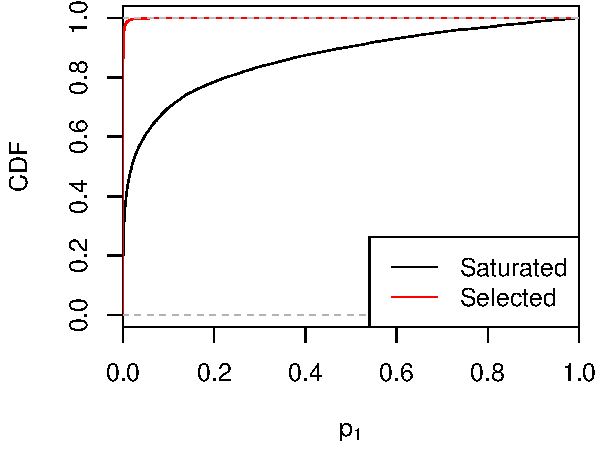
\includegraphics[width=.5\textwidth]{figs/bivariateSelVSat_rocCurve.pdf}
  \caption{\WFcomment{Write caption here.}}
  \label{fig:bv_rocCurve}
\end{figure}

Results in \citet{fithian2014optimal} show that the selected-model test is strictly more powerful when the selected model is correct; i.e., when $\mu_2=0$. Figure~\ref{fig:bv_powCurves_0} shows the power curve for each test when $\mu_2=0$. While the selected-model test is more powerful, the difference between the two is relatively mild. Interestingly, the difference is much more pronounced when $\mu_2=4$, as shown in Figure~\ref{fig:bv_powCurves_4}.

\begin{figure}
  \centering
  \begin{subfigure}[t]{.4\textwidth}
    % source code: bivariateSelVSat.R
    \includegraphics[width=\textwidth]{figs/bivariateSelVSat_powCurves_0.pdf}
    \caption{\WFcomment{Write caption here.}}
    \label{fig:bv_powCurves_0}
  \end{subfigure}
  \hspace{.1\textwidth}
  \begin{subfigure}[t]{.4\textwidth}
    % source code: bivariateSelVSat.R
    \includegraphics[width=\textwidth]{figs/bivariateSelVSat_powCurves_4.pdf}
    \caption{\WFcomment{Write caption here.}}
  \end{subfigure}
  \caption{\WFcomment{Write caption here.}}
   \label{fig:bv_powCurves_4}
\end{figure}



\section{Sequential Inference}

Having discussed methods for constructing single-step $p$-values, we turn now to the problem of constructing a {\em stopping rule}; that is, an estimator $\hk$ of the completion index $k_0(Y)\in \{0,\ldots,d,\infty\}$. $M_k$ is ``rejected'' if and only if $\hk>k$. Thus $\hk$ is the number of models we rejected, while $k_0$ is the number that we should have rejected. The number of type I errors, then, is $(\hk-k_0)_+$, while the number of type II errors is $(k_0-\hk)_+$. Define $V=(\hk-k_0)_+$, the number of excess rejections.

Note that the type I error $V$ is defined in a ``model-centric,'' as opposed to a ``variable-centric,'' fashion: in regression, our model-wise $V$ counts the number of true null {\em models} incorrectly rejected, instead of counting the number of noise variables included in the final model. We can define the (model-wise) familywise error rate (FWER) and false discovery rate (FDR) respectively as $\P_F(V >0)$ and $\E_F[V/(\hk \vee 1)]$. 

We could have instead defined the ``variable-centric'' type I error $\tV$ as the number of noise variables incorrectly included in the final model, with $\tR$ denoting the total number of variables included. Here, by ``noise variable'' we mean one that has a non-zero coefficient in the full model. Using selective inference to control the variable-wise FWER $\P_\mu(\tV>0)$ and FDR $\E[\tV / (\tR \vee 1)]$ is an interesting topic for further study.

\subsection{Stopping Rules}

We will consider stopping rules that depend on the sequence $p_1,\ldots,p_d$ of $p$-values, which have been studied in the literature by \WFcomment{literature review here.} We will focus on three such stopping rules: simple stop, proposed by \WFcomment{whom?}, and the more refined strong stop and forward stop, proposed by \citet{gsell2013sequential}. 

While strong stop and forward stop tend to give more powerful stopping rules, they require independence among the $p$-values. Sections~\ref{sec:modelSPSP}--\ref{sec:pvalSP} discuss conditions on the model sequence $M_{[d]}$ and the $p$-value sequence $p_{[d]}$ under which selective $p$-values are mutually independent. We will see that, typically, selected-model $p$-values are sequentially independent while saturated-model $p$-values are not.

\subsubsection{Basic Stop:}

\WFcomment{Is there a better name for this? Can we find it in the literature?}

The most obvious sequential procedure is to reject at each step until the first time $p_k > \alpha$, which we can formalize as
\[
\hk_B(Y) = \min\left\{k \in \{1,\ldots,m\} :\;
  p_k > \alpha\right\} - 1
\]
We will call this procedure {\em basic stop}. 

If $k_0$ is fixed, then it is clear that $\hk_b$ controls the FWER at level $\alpha$ provided that $p_{k}$ is a valid $p$-value for each $k>k_0$. Then, 
\[
\P(V>0) = \P(p_{k_0+1} \leq \alpha) \leq \alpha.
\]
\WFcomment{Trivial, but no doubt someone else proved this first...}

Selectively valid single-step $p$-values do not necessarily guarantee FWER control when $k_0$ is random. In that case, we need a bit more, but it is sufficient that we have type I error control for $p_k$ conditional on $k_0=k-1$; i.e., not just conditional on $M_{k-1}$ being a correct model, but given that $M_{k-1}$ is the {\em first} correct model.

\subsubsection{Strong Stop:}

\citet{gsell2013sequential} propose another stopping rule that controls the model-wise FWER, which they called {\em strong stop}. Define
\[
  \hk_{S}(Y) = \max\left\{k \in \{1,\ldots,d\} :\;
    \exp\left(\sum_{\ell=k}^d \frac{\log p_\ell}{\ell}\right) 
    \leq \frac{\alpha k}{d}\right\}
\]
Even if $p_k$ is a little larger than $\alpha$, say $\alpha=0.05$ and $p_k=0.06$, strong stop can still reject $M_{k-1}$ if the next three or four $p$-values are also relatively small.

\citet{gsell2013sequential} show that if the completion index $k_0$ is fixed, then $\hk_S$ controls the FWER at level $\alpha$, as long as the null $p$-values are independent given the non-null ones. Specifically, they require that
\begin{equation}\label{eq:indepCond_fixed_k0}
\P(p_{k_0+1} \leq \alpha_{k_0+1}, \ldots, p_d \leq \alpha_d
\mid p_1, \ldots, p_{k_0}) \leq \prod_{\ell=k_0+1}^d \alpha_\ell
\end{equation}

For random $k_0$, it is easy to see that the $p$-values simply need to satisfy~\eqref{eq:indepCond_fixed_k0} conditional on the value of $k_0$:
\begin{equation}\label{eq:indepCond_random_k0}
  \P(p_{k+1} \leq \alpha_{k+1}, \ldots, p_d \leq \alpha_d
  \mid p_1, \ldots, p_{k_0}, \; k_0 = k) \leq \prod_{\ell=k+1}^d \alpha_\ell
\end{equation}
If~\eqref{eq:indepCond_random_k0} holds, then strong stop controls theprobability of $V>0$ conditionally on $k_0$, and thus also marginally.

\subsubsection{Forward Stop:}

\citet{gsell2013sequential} propose another stopping rule, {\em forward stop}, that controls the model-wise FDR:
\[
  \hk_{F}(Y) = \max\left\{k \in \{1,\ldots,d\} :\;
    -\frac{1}{k}\sum_{\ell=1}^k \log(1-p_\ell) \leq \alpha\right\}
\]
If $p_k$ is uniform then  $-\log(1-p_k)$ is an exponential random variable. If all of the null $p$-values are uniform and the others are zero, then only the null ones contribute to the sum, and
\[
\widehat{\text{FDR}}_k = -\frac{1}{k}\sum_{\ell=1}^k \log(1-p_\ell)
\]
is a Gamma random variable with mean $V/k$ and variance $V/k^2$. We stop the last time the estimate of FDR is less than $\alpha$. Forward stop requires the same condition independence condition~\eqref{eq:indepCond_random_k0} as strong stop does.



\begin{comment}

\subsection{Saturated- and Selected-Model $p$-Values in Regression}

If we wish to use strong stop and forward stop, we need the $p$-values to satisfy~\eqref{eq:indepCond_random_k0}, but there is no guarantee that single-step selective $p$-values are independent of each other.

In fact, saturated-model $p$-values typically are not independent. Continuing with Example~\ref{ex:bivariate}, Table~\ref{tab:bv_twoWayTable} shows a two-way contingency table for the saturated-model $p$-values $(p_1(Y), p_2(Y))$, binned into cells of height and width 0.2. Because the global null is true, both $p$-values are uniform by construction, but the $p$-values are strongly dependent, with correlation $-48\%$.

% latex table generated in R 3.0.2 by xtable 1.7-1 package
% Mon May  4 21:11:15 2015
\begin{table}[ht]
  \centering
  \begin{tabular}{l|ccccc|c}
    \multicolumn{7}{c}{Saturated-Model $p$-Values 
      (\% of $10^6$ Simulations)}\\[7pt]
    \hline
    \multicolumn{7}{c}{}\\[-1.5ex]
    \multicolumn{7}{c}{$p_2(Y)$}\\[5pt]
    ${\large p_1(Y)}$ & (0,0.2] & (0.2,0.4] & (0.4,0.6] & (0.6,0.8] & (0.8,1] & \textbf{Total} \\ 
    \hline
    (0,0.2] & 1.0 & 2.7 & 4.2 & 5.6 & 6.7 & 20.1 \\ 
    (0.2,0.4] & 1.4 & 3.4 & 4.5 & 5.2 & 5.5 & 20.0 \\ 
    (0.4,0.6] & 2.3 & 4.3 & 4.7 & 4.5 & 4.2 & 20.0 \\ 
    (0.6,0.8] & 4.2 & 5.4 & 4.3 & 3.4 & 2.7 & 20.0 \\ 
    (0.8,1] & 11.1 & 4.3 & 2.3 & 1.4 & 1.0 & 20.0 \\ 
    \hline
    \textbf{Total} & 19.9 & 20.0 & 20.0 & 20.1 & 20.0 & 100.0 \\ 
    \hline
  \end{tabular}
  \caption{Two-way contingency table of saturated-model $p$-values $(p_1(Y), p_2(Y))$ for Example~\ref{ex:bivariate}, after binning into cells of height and width 0.2. We report the percentage of $p$-value pairs falling into each cell out of one million simulations from the global null hypothesis, $\mu=0$. Both $p$-values are marginally uniform but strongly dependent, with a correlation of $-48\%$.}
\label{tab:bv_twoWayTable}
\end{table}

By contrast, the selected-model $p$-values $(p_1,p_2)$ are independent. To see why, recall that, on the selection event $A$, $p_1$ is only a function of $Y_1$. Moreover, $p_2$ is a selective $p$-value for comparing the null
\[
M_1:\; Y \sim \cN\left(\binom{\mu_1}{0}, I_2\right)
\]
against the alternative
\[
M_2:\; Y \sim \cN\left(\mu, I_2\right), \text{ with } \mu_2 \neq 0.
\]
Because $\mu_1$ is a nuisance parameter in $M_1$, an exact selected-model test must condition on the corresponding sufficient statistic $Y_1$. But that means $p_2$ is uniform given $Y_1$, and therefore also uniform given $p_1(Y_1)$.

A generalization of this argument shows that the $p$-values for the saturated-model tests are always independent:

\begin{proposition}
  The selected-model equal-tailed or UMPU $p$-values after forward-stepwise linear regression. satisfy~\eqref{eq:indepCond_random_k0}.
\end{proposition}
This is a simple consequence of the much more general results proven in Section~\ref{sec:sufficiency}, but it is instructive to see the proof in the relatively concrete case of linear regression.
\begin{proof}
  At step $k$, we are testing the null hypothesis that $\beta_j=0$ in     the model $Y\sim \cN(X_E\beta, I_2)$, for some active set $E\sub [p]$ of size $k$, and some variable $j\in E$. Let $A_{j,E}$ denote the selection event for a particular $j$ and $E$, and let $m_{k-1}(j,E)$ denote the null model with active set $X_{E\setminus j}$.

On $A_{j, E}$, the selected-model $p$-value $p_k$ is based on the null distribution of the test statistic $X_j'Y$ conditional on the null sufficient statistics $X_{E\setminus j}'Y$ and on $Y \in A_{j,E}$.

Moreover, on $A_{j,E}$, the entire sequence of previous $p$-values $p_{[k-1]}$ depend only on the sufficient statistics $X_{E\setminus j}'Y$ of $m_{k-1}(j,E)$. To see why, \WFcomment{complete this proof.}

We have shown that, if $m_{k-1}(j,E)$ is true, then $p_k$ is uniform and independent of $p_{[k-1]}$ on $A_{j,E}$ for each $j$ and $E$. That is,
\[
\P_F\left(p_{k} \leq \alpha \mid p_{[k-1]}, Y \in A_{j,E} \right) = \alpha \quad \forall F \in m_{k-1}.
\]
It follows that 
\[
\P_F\left(p_{k} \leq \alpha \mid p_{[k-1]}, F \in M_{k-1} \right) = \alpha \quad \forall F.
\]
\end{proof}
The proof turns on two properties of selected-model $p$-values, and one property of forward stepwise regression. 

As for the $p$-values, we used the fact that $p_{k,m_{k-1},m_k}$ is uniform conditional on the sufficient statistics of the null model $m_{k-1}$. This is true for selected-model and saturated-model $p$-values alike. We also used the fact that $p_{k,m_{k-1},m_k}$ follows the {\em sufficiency principle} --- that is, it depends only on the sufficient statistics of $m_k$. This is {\em not} true of the saturated-model $p$-values: to compute them, we must know $\proj_{\eta}^\perp Y$, which depends on statistics that are ancillary for $m_{k-1}$.

We also used the fact that, in the forward stepwise algorithm, if $m_k$ is the $k$th model then, on the event $M_k=m_k$, all the models up to step $k$ depend only on sufficient statistics of $m_k$. This is a sort of {\em sub-path sufficiency principle} which many other algorithms satisfy, as we will see in Section~\ref{sec:modelSPSP}.

\subsection{Conditions for Independent $p$-Values}\label{sec:sufficiency}

To obtain a sequence of $p$-values, we must specify what model selection algorithm $M_{[d]}$ to use, as well as how to construct $p$-values at each step. In this section we consider what conditions are sufficient to guarantee that the resulting $p$-value sequence is independent. 

\begin{comment}
Sections~\ref{sec:pvalSP}--\ref{sec:modelSPSP} discuss sufficient conditions on the $p$-values and the selection algorithm under which single-step $p$-values are automatically independent. Section~\ref{sec:selectionVariables} discusses how we can create independent $p$-values by conditioning on finer selection variables at each step.

Essentially, we will want to partition the information in $Y$ according to the filtration:
\begin{align}\nonumber
  \sF(M_0,T_0) &\underlabel_{\text{selection } 1} 
  \sF(M_{[1]},T_0) \underlabel_{\text{inference } 1}
  \sF(M_{[1]},T_1) \quad \sub \;\;\cdots\\[8pt]
  \label{eq:infoPartition}
  \cdots\;\; \sub \quad&
  \sF(M_{[d-1]},T_{d-1}) \underlabel_{\text{selection } d}
  \sF(M_{[d]},T_{d-1}) 
  \underlabel_{\text{inference } d}
  \sF(M_{[d]}, T_d)
\end{align}
\end{comment}

\subsubsection{Independent $p$-Values and the Sufficiency Principle}\label{sec:pvalSP}

Assume that every candidate model $m$ has a set of minimal sufficient statistics $T(y; \;m)$. For linear regression, the sufficient statistics for $M(E)$ are $X_E'Y$ if $\sigma^2$ is known and  $(X_E'Y,\|Y\|)$ otherwise. At step $k$, let $T_k(Y) = T(Y; \;M_k(Y))$ denote the sufficient statistics for the model actually chosen --- for example, $X_{E_k(Y)}'Y$.

For a candidate pair $(m_{k-1},m_k)$ of models to test at step $k$, define the selection event $A = \{M_{k-1} = m_{k-1}, M_k=m_k\}$. The $p$-value for this pair, $p_{k,m_{k-1},m_k}$ satisfies the sufficiency principle if 
\[
\P_F\left(p_{k,m_{k-1},m_k}(Y) \mid M_{k-1}=m_{k-1}, M_k=m_k\right)
\]
This is what we mean when we say $p_{k,m_{k-1},m}$ is ``based on'' the law
\[
\L_{m_{k-1}}\left(T_k \;\;\mid\;\; T_{k-1},\; M_{k-1}=m_{k-1},\;M_k=m_k\right)
\]
for some minimal sufficient statistics $T_{k-1}(Y)$ and $T_k(Y)$ of $m_{k-1}$ and $m_k$, respectively. More precisely, $p(Y)$ must be uniform or conservative conditional on $T_{k-1}(Y)$, and it must be a function of $T_k(Y)$ on $A$.

\subsubsection{A Sub-Path Sufficiency Principle for Model Selection Procedures}\label{sec:modelSPSP}

We say that a selection algorithm $M_{[d]}(\cdot)$ satisfies the {\em sub-path sufficiency principle} (henceforth SPSP) if, on the event $M_k(Y)=m_k$, the sequence of models $M_{[k]}$ depends only on sufficient statistics of $m_k$. Again, if 

It will be useful to introduce the following notation:

\begin{model}[Generalized Sparse Model]\label{mod:genSparse}
  Let $M$ be a model parameterized by $\theta\in \Theta \sub \R^p$:
  \[
  M = \{F_\theta:\; \theta \in \Theta\}.
  \]
  For subsets $E\sub [p]$ define the submodel with active coefficients $E$ as follows:
  \[
  \Theta(E) = \{\theta:\; \theta_j = 0, \;\;\forall j \notin E\}, 
  \quad M(E) = \{F_\theta:\; \theta\in \Theta_E\}.
  \]
  Let $L(\theta; Y)$ denote the likelihood for model $M$.
\end{model}
Note that, although we will make no assumptions about the form of $M$, the results of this section are only useful in cases where we can actually construct single-step $p$-values. At present, that caveat largely restricts us to using exponential family models.

In Model~\ref{mod:genSparse}, the {\em forward stepwise} algorithm proceeds as follows: we first set $E_0(Y)$ arbitrarily, then at step $k=1,\ldots,d$, we define
\begin{align}\label{eq:forwardDef_start}
j_k &= \argmax_j \;\;\sup \left\{L(\theta; Y):\; \theta\in\Theta(E_{k-1} \cup \{j\})\right\} \\
E_k &= E_{k-1} \cup \{j_k\}\\\label{eq:forwardDef_end}
M_k &= M(E_k)
\end{align}

To make this definition more concrete, we can specialize it to several familiar examples:

\begin{example}[Forward Stepwise Regression]
In the case of linear regression with known $\sigma^2$, $p$ is the number of variables and $M$ is $\cN(X\beta, \;\sigma^2I)$. For active set $E \sub [p]$, $M(E)$ is the model $\cN(X_E\beta_E, \;\sigma^2I)$, and $E_0 = \emptyset$. Because the maximized log-likelihood for a linear regression is monotone in the residual sum of squares, the forward stepwise algorithm adds whichever variable reduces the residual sum of squares the most.

For linear regression with unknown $\sigma^2$, there are $p+1$ parameters $(\beta, \sigma^2)$ and $E_0 = \{p+1\}$ because $\sigma^2$ is a parameter for every model.
\end{example}

\begin{example}[Principle Components Analysis]
\WFcomment{Do this one.}  
\end{example}

All forward stepwise procedures satisfy the SPSP.

\begin{proposition}[Forward Stepwise Satisfies SPSP]\label{prop:forwardSPSP}
  The forward stepwise algorithm in Model~\ref{mod:genSparse} as defined in (\ref{eq:forwardDef_start}--\ref{eq:forwardDef_end}) satisfies the SPSP.
\end{proposition}
\begin{proof}
  Let $A$ denote the event $\{M_k = M(E)\}$ for some fixed active set $E$. Letting $T(Y)$ be a sufficient statistic for $m_k$, the likelihood $L$ restricted to $\Theta(E) \times A$ is proportional to a function depending only on $T$. If $L_T$ is the likelihood of $T(Y)$, then
\[
L(\theta; y) = L_T(\theta; T(y)) \;L_{Y\mid T}(y), \;\; \text{ for } (\theta, y) \in  \Theta(E) \times A.
\]
Note that $L_{Y \mid T}(y)$ does not depend on $\theta$ since $T$ is sufficient for $M(E)$.

For $y\in A$ and $\ell \leq k$, we have $E_\ell(y) \sub E$. This means that the maximizer in \eqref{eq:forwardDef_start} is attained for some $j\in E$. So, for $\ell \leq k$, on $A$,
\begin{align}
  j_\ell &= \argmax_{j\in E} \;\;\sup \left\{L(\theta; Y):\;
    \theta\in\Theta(E_{\ell-1} \cup \{j\})\right\} \\
  &= \argmax_{j\in E} \;\;\sup \left\{L_T(\theta; T(Y)):\;
    \theta\in\Theta(E_{\ell-1} \cup \{j\})\right\}. \label{eq:onlyT}
\end{align}
Replacing $L$ with $L_T$ in~\eqref{eq:onlyT} is justified because $\Theta(E_{\ell - 1} \cup \{j\}) \sub \Theta(E)$ when $E_{\ell-1}\cup E$ and $j\in E$.

Equation~\eqref{eq:onlyT} shows that $j_1,\ldots, j_{k-1}$ all depend on $Y$ only through $T(Y)$. As a result, it also follows that the sequence $M_{[k-1]}(Y)$ depends only of $T(Y)$.
\end{proof}

Another class of model selection procedures satisfying the SPSP is the sequence ``ever-active'' sets in regularized likelihood methods. For $r=0,1,\ldots$, let $P_r(\theta)$ denote a regularizing penalty, and define
\begin{align}\label{eq:regPathDef_start}
  \hat\theta^{r}(Y) &= 
  \argmin_{\theta\in\Theta} -\log L(\theta; Y) + P_r(\theta) \\
  \tE_r(Y) &= \left\{j:\; \hat\theta_j^s \neq 0 
    \text{ for any } s \leq r \right\}
\end{align}

While the sets $\tE_r$ are nested by definition, we could have $\tE_r = \tE_{r+1}$ for most values of $r$. We will take the sequence of {\em distinct} ever-active sets. Let $R_0=0$, and for $k>0$ let $R_k$ denote the (random) index where the active set actually changes:
\begin{align}
  R_k &= \min\{s:\; \tE_s \neq \tE_{R_{k-1}}\}\\
  E_k &= \tE_{R_k}\\
  \label{eq:regPathDef_end}
  M_k &= M(E_k)
\end{align}
\WFcomment{Slightly sloppy definitions: note that $d$, the number of models, is random. $d$ could be 0 or could be infinite, depending on the data. Also, it isn't really necessary that the $r$ values be integers...}

\begin{proposition}[Regularized Likelihood Paths Satisfy SPSP]\label{prop:regPathSPSP}
Ever-active model paths derived from regularized likelihood methods as in (\ref{eq:regPathDef_start}--\ref{eq:regPathDef_end}) satisfy the sub-path sufficiency principle.
\end{proposition}

\begin{proof}
  Again, let $A$ denote the event $\{M_k = M(E)\}$ for some fixed $E$, and define $T$ and $L_T$ as in the proof of Proposition~\ref{prop:forwardSPSP}. We can partition $A$ into subsets $A_r = A \cap \{R(k)=r\}$.

On the event $A_r$, every $\hat\theta^s$ for $s\leq r$ is supported on $E$. That is, for $s \leq r$, we can write 
\begin{equation}\label{eq:onlyT_Ar}
  \hat\theta^{s} = 
  \argmin_{\theta\in\Theta(E)} -\log L_T(\theta; T(Y)) + P_s(\theta) \quad \text{ on } A_r
\end{equation}
Equation~\label{eq:onlyT_Ar} guarantees that $M_{[k-1]}$ is a function of $T(Y)$ on $A_r$. That is, we can write
\[
M_{[k-1]}(Y) = M_{[k-1]}^r(T(Y)) \quad \text{ on } A_r
\]
It remains only to show that, on $A$, $R_k(Y)$ depends only on $T(Y)$; then we have
\[
M_{[k-1]}(Y) = M_{[k-1]}^{R(T)}(T) \quad \text{ on } A
\]
But $R_k$ is a function of $T$ on $A$ for the same reason: that $\hat\theta^s$ depends only on $T$ until other coefficients enter the model.
\WFcomment{Would the proof be cleaner with $A_r$ defined as $A\cap \{R_k \leq r\}$?}
\end{proof}

\begin{comment}
\WFcomment{There is a filtration interpretation when you have the appropriate sufficiency properties.} Let $\sF_{k,\ell}$ denote the $\sigma$-algebra generated by $M_{[k]}$ and $p_{[\ell]}$.
\begin{align*}
  \sF_{k,\ell} &= \sF(M_{[k]},p_{[\ell]})\\
  \sF_0 &\underlabel_{\text{selection } 1} \sF_{1,0} \underlabel_{\text{inference } 1}
  \sF_{1,1} \;\;\sub \cdots \sub\;\;
  \sF_{d-1,d-1} \underlabel_{\text{selection } d} \sF_{d,d-1}
  \underlabel_{\text{inference } d} \sF_{d,d}
\end{align*}
\end{comment}

\subsection{Independent $p$-Values Via Selection Variables}\label{sec:selectionVariables}

As discussed in \citet{fithian2014optimal}, there are occasions when it is desirable for some reason to condition on more than just the selection event. On these occasions we can introduce a {\em selection variable} --- any random variable that is finer than the indicator of the selection event --- and condition on its value. Conditioning on a finer selection variable preserves validity conditional on the selection event, but tends to reduce the power of a test. 

For example, in linear regression after selecting variables via the lasso, \citet{lee2013exact} propose conditioning not only on the set of active variables but also on the signs of the active coefficients. The selection event corresponding to a given active set $E\sub [p]$ typically contains up to $2^{|E|}$ convex polytopes, each of which corresponds to a particular sign pattern $\hat z_E$. Thus, conditioning on the selection variable $\hat z_E$ can simplify computation considerably.

We say that $p_{k,m_{k-1},m_k}$ is a selective $p$-value with respect to selection variable $S(Y)$ if it is uniform under $F\in m_k$ given $S$. 

To achieve joint error control properties among different tests, we may need to condition on a finer variable.
\end{comment}

\section{Simulation: Sparse Linear Regression}\label{sec:sparseReg}

Next we compare several model selection procedures in simulation. We simlate from a linear regression model with $n=100$ observations and $p=40$ variables. The design matrix $X\in\R^{n\times p}$ is a random Gaussian design with pairwise correlations of 0.3 between predictor variables.

The columns of $X$ are normalized to have length 1, and we simulate from $Y \sim \cN(X\beta,I_n)$, using a seven-sparse model with signal-to-noise ratio 5:
\[
\beta_j = \left\{\begin{matrix}5 & j = 1,\ldots,7\\ 0 &
    j>7\end{matrix}\right.
\]
We use known $\sigma^2=1$, so that we can compare the saturated-model test with the selected-model test. For our selection algorithm, we use the entire forward-stepwise path, for all 40 steps. 

\subsection{Single-Step $p$-Values}

For each step we compute one-step selected-model and saturated-model $p$-values, as well as nominal (unadjusted) $p$-values, conditioning on the signs of the active variables to make the problem more computationally tractable. Figure~\ref{fig:simulation_null_false} shows the power of all three tests for each of the first ten steps, conditional on the event that the null hypothesis is false. It is clear from Figure~\ref{fig:simulation_null_false} that the selected-model $p$-values are far more powerful than the saturated-model $p$-values. The nominal $p$-values are also quite powerful, but they do not have the correct level.

\begin{figure}
  \centering
  % source code: ??? for simulation, sparseSim.R for plotting
  \includegraphics[width=.8\textwidth]{figs/simulation_snr_5_alpha_05_null_false.pdf}
  \caption{CDFs of saturated-model (black), selected-model (red), and nominal (blue) $p$-values in the simulation of Section~\ref{sec:sparseReg}, conditional on testing a false null hypothesis at step $k$. The selected-model test is much more powerful than the saturated-model test. The nominal test appears powerful, but is not a correct $p$-value.}
  \label{fig:simulation_null_false}
\end{figure}

\begin{figure}
  \centering
  % source code: ??? for simulation, sparseSim.R for plotting
  \includegraphics[width=.8\textwidth]{figs/simulation_snr_5_alpha_05_null_true.pdf}
  \caption{CDFs of saturated-model (black), selected-model (red), and nominal (blue) $p$-values in the simulation of Section~\ref{sec:sparseReg}, conditional on testing a true null hypothesis at step $k$. The selected-model test is much more powerful than the saturated-model test. The nominal test is badly anti-conservative.}
  \label{fig:simulation_null_true}
\end{figure}

\begin{figure}
  \centering
  % source code: ??? for simulation, sparseSim.R for plotting
  \includegraphics[width=.8\textwidth]{figs/simulation_snr_5_alpha_05_noise_var.pdf}
  \caption{CDFs of saturated-model (black), selected-model (red), and nominal (blue) $p$-values in the simulation of Section~\ref{sec:sparseReg}, conditional on the event that the variable added at step $k$ is a noise variable in the full model. Here, none of the methods produce uniform $p$-values. The null hypothesis is false in most cases and so --- in our model-centric point of view --- rejection is the desired outcome.}
  \label{fig:simulation_noise_var}
\end{figure}

Figure~\ref{fig:simulation_null_true} shows the distribution of $p_k$ for $k = 8, \ldots, 17$, given that the null hypothesis tested at step $k$ is correct (i.e., that $k_0< k$). Because the correct model is seven-sparse, $k=8$ is the first index for which the null can possibly be true. Both selective $p$-values are uniform by construction, but the nominal $p$-values are highly anti-conservative, as expected.

Finally, as a warning against misinterpretation of our method, we include Figure~\ref{fig:simulation_noise_var} showing the first ten $p$-values for each method, conditional on event that the variable added at step $k$ is a noise variable in the full model. Now, none of the $p$-values are uniform. 

This is {\em not} a mistake in our implementation of the method, but rather a consequence of our ``model-centric'' point of view. If we try to add a noise variable to the model before we have included all the signal variables, then we are testing a false null hypothesis. The test rejects because there is much more signal to find, and as such, it is entirely appropriate for us to reject the null and continue growing the model.

\subsection{Model-Selection Performance}

If we combine the saturated-model or selected-model $p$-values with one of our three stopping rules, we can evaluate the model-selection performance of each method in terms of:
\begin{itemize}
\item its probability of selecting a correct model or $p_{\text{screen}}$,
\item its model-wise FWER,
\item its model-wise FDR, and
\item its variable-wise FDR, where we use $\tV= \#\{\text{ noise variables included in } M_{\hk}\}$ instead of $V=(\hk-k_0)_+$.
\end{itemize} 
The last measure of performance is not explicitly controlled by any of the selective-inference methods, but we might nevertheless hope to perform reasonably. \WFcomment{Comment on results once they are correct. These numbers are wrong right now.}

\WFcomment{Should we compute the FWER and FDR only conditional on screening? Strong / Forward / Simple should all be correct given screening since they condition on $p_{[k_0-1]}$.}

% latex table generated in R 3.0.2 by xtable 1.7-1 package
% Fri May  1 09:29:28 2015
\begin{table}[ht]
  \centering
  \begin{tabular}{llcccc}
    \hline
    Method & Stopping Rule & $p_{\text{screen}}$ & $\text{FWER}_{\text{mod}}$ 
    & $\text{FDR}_{\text{mod}}$ 
    & $\text{FDR}_{\text{var}}$ \\ 
    \hline
    Selected & Basic & .290 & .000 & .002 & .039 \\ 
    Selected & Forward & .559 & .027 & .020 & .066 \\ 
    Selected & Strong & .041 & .014 & .008 & .042 \\ 
    \hline
    Saturated & Basic & .000 & .000 & .000 & .028 \\ 
    Saturated & Forward & .014 & .000 & .000 & .030 \\ 
    Saturated & Strong & .000 & .000 & .000 & .032 \\ 
    \hline
    Knockoffs & & .000 & --- & --- & .231 \\ 
    \hline
  \end{tabular}
  \caption{\WFcomment{Comment on results once they are correct. These numbers are wrong right now.}}
\end{table}



\section{Simulation: Principal Components Analysis}\label{sec:pca}

\WFcomment{Can we do this one?}


\section{Discussion}


\bibliographystyle{plainnat}
\bibliography{biblio}

\end{document}
